\documentclass[]{report}

\usepackage{hyperref}
\usepackage{float}
\usepackage{needspace}
\usepackage{interval}
\usepackage{pgfplots}
\usepackage{neuralnetwork}
\usepackage[utf8]{inputenc}
\usepackage[T1]{fontenc}
\usepackage[a4paper, left=2.5cm, right=2.5cm, top=2cm, bottom=2cm]{geometry}

\hypersetup{
    colorlinks=true,
    linkcolor=blue,
    filecolor=magenta,      
    urlcolor=black,
}

\renewcommand{\thesection}{\Alph{section}}
\renewcommand{\thesubsection}{\arabic{subsection}}
\renewcommand{\thesubsubsection}{(\emph{\alph{subsubsection}})}

\title{The math behind an artificial neural network}
\author{Hugo Lageneste}
\date{January 2020}

\begin{document}

\begin{titlepage}
    \center
    
    \newcommand{\HRule}{\rule{\linewidth}{0.5mm}}
    \HRule \\[0.4cm]
    {\huge \bfseries The math behind an artificial neural network  }\\[0.1cm]
    \HRule \\[0.4cm]
    
    {Hugo \textsc{Lageneste}}\\[0.5cm]
    {\large January 2020}\\[2cm]
    
    \vfill
    \begin{neuralnetwork}[height=10, nodespacing=25mm, layerspacing=35mm, nodesize=30pt]
        \inputlayer[count=5, bias=false]
        \hiddenlayer[count=6, bias=false]
        \linklayers
        \hiddenlayer[count=6, bias=false]
        \linklayers
        \outputlayer[count=3]
        \linklayers
    \end{neuralnetwork}
    \vfill
\end{titlepage}

\begingroup
\let\cleardoublepage\relax
\let\clearpage\relax

\tableofcontents

\needspace{6cm}
\[\;\]

\vfill

\endgroup

\chapter*{The math behind an artificial neural network}

\setcounter{section}{-1}
\section{Introduction}
\label{sec:intro}

\subsection{Application example}

{Let's take an example to see how an ANN\footnote{Artificial Neural Network} works.}

\begin{figure}[H]
    \centering
    \begin{tabular}{|l|c|c|r|}
      \hline
      Obesity & Exercise & Smoking & Diabetic \\
      \hline
      1 & 0 & 0 & 1 \\
      0 & 1 & 0 & 0 \\
      0 & 0 & 1 & 0 \\
      1 & 1 & 0 & 1 \\
      \hline
    \end{tabular}
    \caption{Example of a set of persons with Obesity, Exercise, Smoking and Diabetic properties. The 1 stands for true, the 0 for false.}
\end{figure}

{We can observe that in this example, a person with diabetes is inevitably obese. What if we want a program which takes in parameter those 4 examples and can predict if a person is diabetic or not?}\\

{This problem can be modeled as an ANN with 3 input nodes which represent each property: the Obesity, Exercise and Smoking and a single output node which represents
the Diabetic column.}

\begin{figure}[H]
    \centering
    \begin{neuralnetwork}[height=3, nodespacing=15mm]
        \inputlayer[count=3, bias=false, title=Input layer]
        \outputlayer[count=1, title=Output layer]
        \linklayers
    \end{neuralnetwork}
    \caption{Diagram of the ANN to model the example}
\end{figure}

\subsection{Neural network operation}
\label{subsec:operation}

{Each property is represented as an input node so the network will operate as a function to say if the person is diabetic or not. The input nodes from a same layer are not link together but each node is linked to every node from the previous layer and from the next layer. Links between nodes are represented as weights and are unique to each liaison. A unique value is held in each node which is calculated with previous nodes values and weights. The whole goal of the neural network is to adjust the weights to make the final predictions
right.}\\

{To adjust the weights, we will proceed in different steps. First of all, the neural network will
compute the output values named the prediction. Then, the network will use a function to calculate the error of accuracy and adjust the weights. This process will be repeated until the success rate is convenient.}

\section{Forward propagation}

{As seen in the Introduction \ref{sec:intro}, each node holds a value contained between 0 and 1, and calculated with values of the previous neurons, weights and biases.}

\begin{figure}[H]
    \centering
    \begin{neuralnetwork}[height=4, nodespacing=15mm]
        \newcommand{\inputtext}[2]{$a^{(l-1)}_#2$}
        \newcommand{\outputtext}[2]{$a^{(l)}_#2$}
        \inputlayer[count=3, bias=false, text=\inputtext, title=Input layer]
        \outputlayer[count=1,  text=\outputtext, title=Output layer]
        \linklayers[title=Weights $w_k$]
    \end{neuralnetwork}
    \caption{Diagram of a neural network, $a$ is a node's value, its exponent represents the index of the layer and its subscript the index of the neuron then.}
\end{figure}

{Let $z^{(l)}_1$ be the sum of the bias and the dot product of weights $w_k$ and values of the previous neurons $a^{(l-1)}_k$.}

\[{z^{(l)}_1=b^{(l)}_1+\sum_{k=1}^{n_{(l-1)}} a^{(l-1)}_k w_k}\]

{In order to keep the values in the neurons between 0 and 1, we are going to use the sigmoid function which is defined on $\interval[open]{0}{1}$, noted :}
\[\sigma(x)=\frac{1}{1+e^{-x}}\]

\begin{figure}[H]
    \centering
    \begin{tikzpicture}
        \begin{axis}[grid=major, xmax=6, ymax=1.1, samples=50, xlabel=$x$, ylabel=$\sigma(x)$]
          \addplot[black, thin] (x,1/(1+e^(-x)));
        \end{axis}
    \end{tikzpicture}
    \caption{Graphical representation of the sigmoid function}
\end{figure}

{Thus,}

\[a^{(l)}_1=\sigma\left(z^{(l)}_1\right)\]
\[a^{(l)}_1 \in \interval[open]{0}{1}\]

{This calculus can be visualised with matrix too}

\[a^{(l)}_1=\sigma\left(\begin{bmatrix}w_1 & w_2 & w_3\end{bmatrix}\begin{bmatrix}a^{(l-1)}_1 \\ a^{(l-1)}_2 \\ a^{(l-1)}_3\end{bmatrix}+\begin{bmatrix}b^{(l)}_1\end{bmatrix}\right)\]

\section{Back propagation}

\subsection{Cost function}

{Let's take a simple example of a one-input-layer-one-output-layer-neural-network}

\begin{figure}[H]
    \centering
    \begin{neuralnetwork}[height=2, nodespacing=15mm]
        \newcommand{\inputtext}[2]{$a^{(l-1)}$}
        \newcommand{\outputtext}[2]{$a^{(l)}$}
        \inputlayer[count=1, bias=false, text=\inputtext, title=Input layer]
        \outputlayer[count=1,  text=\outputtext, title=Output layer]
        \linklayers[title=Weight $w$]
    \end{neuralnetwork}
    \caption{Diagram of the ANN to model the example of the cost function}
    \label{fig:simplenn}
\end{figure}

{Once again,}

\[z^{(l)}=b+a^{(l-1)}w\]
\[a^{(l)}=\sigma\left(z^{(l)}\right)\]

{The goal is now to adjust the weights to make the predictions more accurate. Let $C_1$ be the cost function/error function which is the square difference between the prediction and the actual output $y$.}

\[C_1\left(a^{(l)},y\right)=\left(a^{(l)}-y\right)^2\]

{The smaller the cost function is, the more accurate the predictions are, mathematically the goal is to minimize the cost function.}

\begin{figure}[H]
    \centering
    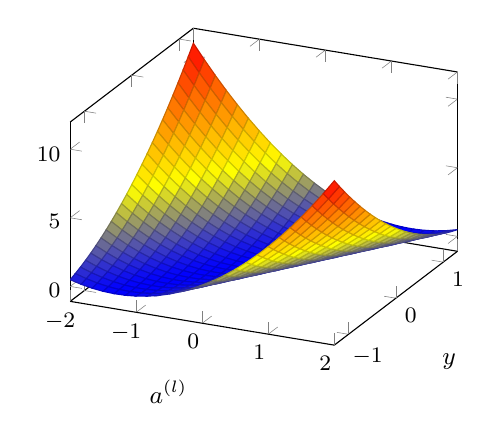
\begin{tikzpicture}
        \begin{axis}[
            xlabel=$a^{(l)}$, ylabel=$y$,
        	small,
        ]
        \addplot3[
        	surf,
        	domain=-2:2,
        	domain y=-1.3:1.3,
        ] 
        	{(x-y)^2};
        \end{axis}
    \end{tikzpicture}
    \caption{Graphical representation of cost function from the previous neural network, figure \ref{fig:simplenn}}
\end{figure}

\subsection{Gradient descent}

{Now we will need to understand how sensitive the cost function is to small changes to $w_k$ because remember from \ref{subsec:operation}, the goal is to adjust weights. Thus, we will determine the partial derivative of $C$ with respect to $w$ using the chain rule.}

\[{\frac{\partial C_1}{\partial w}=\frac{\partial C_1}{\partial a^{(l)}} \frac{\partial a^{(l)}}{\partial z^{(l)}} \frac{\partial  z^{(l)}}{\partial w}}\]

{Indeed,}

\[\frac{\partial C_1}{\partial a^{(l)}}=2\left(a^{(l)}-y\right)\]
\[\frac{\partial a^{(l)}}{\partial z^{(l)}}=\frac{\partial \sigma\left(z^{(l)}\right)}{\partial z^{(l)}}=\sigma\prime\left(z^{(l)}\right)\]
\[\frac{\partial  z^{(l)}}{\partial w}=\frac{\partial  \left(b+a^{(l-1)}w\right)}{\partial w}=a^{(l-1)}\]

{All together, it gives us}

\[\frac{\partial C_1}{\partial w}=2\left(a^{(l)}-y\right) \sigma\prime\left(z^{(l)}\right) a^{(l-1)}\]

{We will use this formula to calculate the adjustments to make to the weights multiple times until the predictions are accurate.}

\section{Complex example}

\begin{figure}[H]
    \centering
    \begin{neuralnetwork}[height=4, nodespacing=15mm]
        \newcommand{\inputtext}[2]{$a^{(l-1)}_#2$}
        \newcommand{\outputtext}[2]{$a^{(l)}_#2$}
        \inputlayer[count=3, bias=false, text=\inputtext, title=Input layer $a^{(l-1)}_k$]
        \outputlayer[count=2,  text=\outputtext, title=Output layer $a^{(l)}_j$]
        \linklayers[title=Weight $w_{jk}$]
    \end{neuralnetwork}
    \caption{Diagram of a more complex ANN}
\end{figure}

{We will model this problem with matrix because it is easier}

\subsection{Forward propagation}

{First of all we are going to create a matrix of weights and of bias}

\[w=\begin{bmatrix}
w_{11} & w_{21} \\
w_{12} & w_{22} \\
w_{13} & w_{23} \\
\end{bmatrix}\]
\[b=\begin{bmatrix}
b_{1} & b_{2} \\
b_{1} & b_{2} \\
b_{1} & b_{2} \\
\end{bmatrix}\]

{Then, let's calculate the predictions $a$. We consider that we have 3 set of input examples.}

\[z=\begin{bmatrix}
a^{(l-1)}_1 & a^{(l-1)}_2 & a^{(l-1)}_3 \\
\ldots & \ldots & \ldots \\
\ldots & \ldots & \ldots \\
\end{bmatrix}\cdot w+b\]
\[a=\sigma (z)\]

\subsection{Back propagation}

{We will use the cost function derivative to calculate the adjustments to make to the weights}

\[e=a-\begin{bmatrix}
a^{(l)}_1 & a^{(l)}_2 \\
\ldots & \ldots \\
\ldots & \ldots \\
\end{bmatrix}\]
\[w_{adj}=2e \cdot \sigma\prime (z)\cdot
\begin{bmatrix}
a^{(l-1)}_1 & a^{(l-1)}_2 & a^{(l-1)}_3 \\
\ldots & \ldots & \ldots \\
\ldots & \ldots & \ldots \\
\end{bmatrix}\]

{We can now add up the adjustments to the weights}

\[w=w+w_{adj}\]

{And repeat the process until the success rate is >95\%}

\end{document}
